\documentclass[xetex,mathserif,serif]{beamer}
\usepackage{polyglossia}
\setdefaultlanguage[babelshorthands=true]{russian}
\usepackage{minted}
\usepackage{tabu}

\useoutertheme{infolines}

\usepackage{fontspec}
\setmainfont{FreeSans}
\newfontfamily{\russianfonttt}{FreeSans}

\usepackage{textpos}
\setlength{\TPHorizModule}{1cm}
\setlength{\TPVertModule}{1cm}

\setbeamertemplate{blocks}[rounded][shadow=false]

\setbeamercolor*{block title alerted}{fg=red!50!black,bg=red!20}
\setbeamercolor*{block body alerted}{fg=black,bg=red!10}

\tabulinesep=1.2mm

\title{Занятие 2: работа с требованиями}
\author[Юрий Литвинов]{Юрий Литвинов\\\small{\textcolor{gray}{yurii.litvinov@gmail.com}}}
\date{20.09.2017}

\newcommand{\todo}[1] {
	\begin{center}\textcolor{red}{TODO: #1}\end{center}
}

\newcommand{\DownArrow} {
	\hspace{2cm}\begin{LARGE}$\downarrow$\end{LARGE}
}

\newcommand{\attribution}[1] {
	\begin{flushright}\begin{scriptsize}\textcolor{gray}{\textcopyright\; #1}\end{scriptsize}\end{flushright}
}

\begin{document}

	\frame{\titlepage}

	\section{Введение}

	\begin{frame}
		\frametitle{Требования}
		\begin{itemize}
			\item Функциональные --- то, \emph{что} система должна делать
			\item Нефункциональные --- то, \emph{как} система должна это делать
			\begin{itemize}
				\item Эффективность
				\item Масштабируемость
				\item Удобство использования
				\item Надёжность
				\item Безопасность
				\item Сопровождаемость и расширяемость
				\item ...
			\end{itemize}
			\item Ограничения
			\begin{itemize}
				\item Технические
				\item Бизнес-ограничения
			\end{itemize}
		\end{itemize}
	\end{frame}

	\section{Инструменты для работы с требованиями}

	\begin{frame}
		\frametitle{Метод случаев использования}
		Разработан Иваром Якобсоном в 1992 году как средство для анализа требований
		\begin{itemize}
			\item Акторы
			\begin{itemize}
				\item Роль пользователя системы
				\item Может быть не только группой людей, но и внешней системой
			\end{itemize}
			\item Случаи использования
			\begin{itemize}
				\item Полезная функция системы
				\item Раскрывается в набор сценариев использования, которые описываются текстом или в виде диаграмм активностей
			\end{itemize}
			\item Граница системы
			\begin{itemize}
				\item Отделяет то, что внутри, от того, что вне
			\end{itemize}
		\end{itemize}
		Диаграммы случаев использования включены в UML
	\end{frame}

	\begin{frame}
		\frametitle{Диаграммы случаев использования}
		\begin{center}
			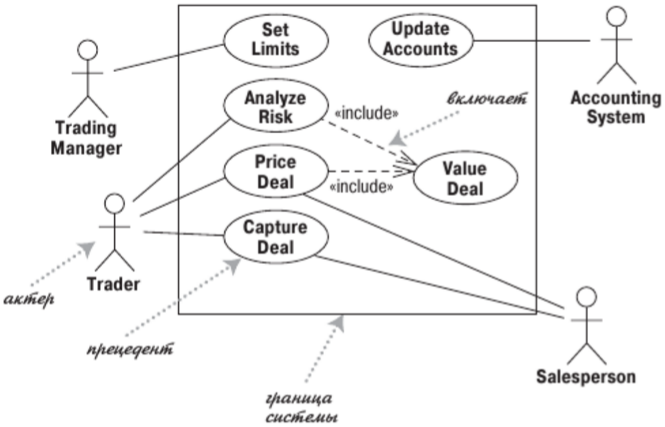
\includegraphics[width=0.5\textwidth]{useCaseDiagram.png}
		\end{center}
		\attribution{М. Фаулер, ``UML. Основы''}
	\end{frame}

	\begin{frame}
		\frametitle{Диаграммы активностей}
		\begin{center}
			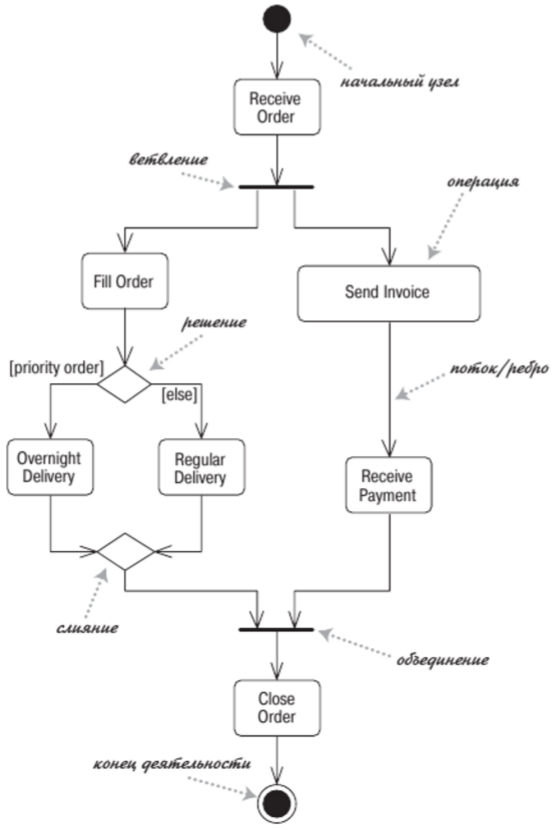
\includegraphics[width=0.35\textwidth]{activityDiagram.png}
		\end{center}
		\attribution{М. Фаулер, ``UML. Основы''}
	\end{frame}

	\begin{frame}
		\frametitle{Диаграммы требований SysML}
		\begin{center}
			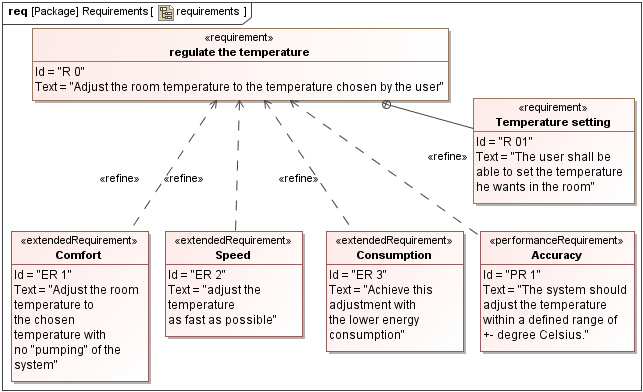
\includegraphics[width=0.75\textwidth]{sysMlRequirementDiagram.png}
		\end{center}
		\attribution{``No Magic'' documentation}
	\end{frame}

	\begin{frame}
		\frametitle{Feature-Oriented Domain Analysis}
		\begin{itemize}
			\item 1990 год, SEI
			\item Прежде всего, для разработки линеек продуктов
			\item Строится модель предметной области в виде диаграммы характеристик
			\item Характеристики используются, чтобы сконфигурировать готовую систему
			\begin{itemize}
				\item Прежде всего, чтобы обеспечить переиспользование
				\item Простая нотация для визуализации фич и отношений между ними
			\end{itemize}
		\end{itemize}
	\end{frame}

	\begin{frame}
		\frametitle{Feature Diagrams}
		\begin{center}
			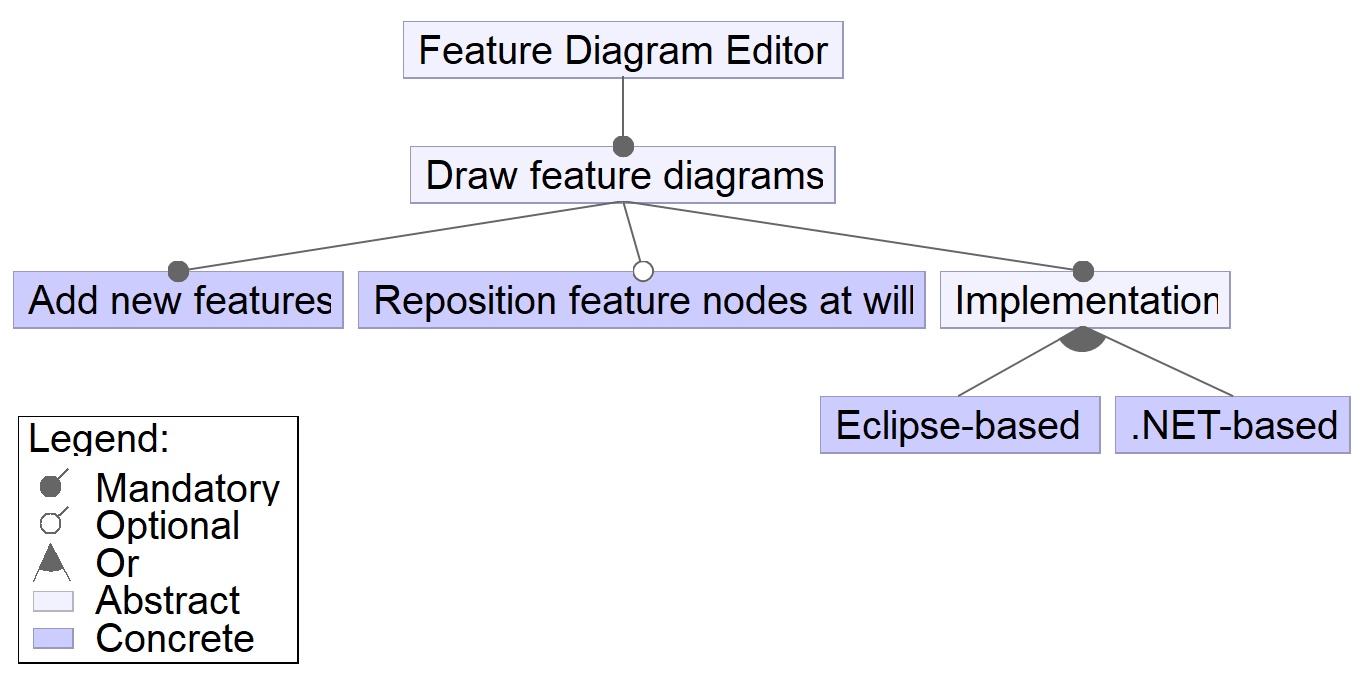
\includegraphics[width=0.9\textwidth]{featureDiagram.png}
		\end{center}
		\begin{footnotesize}
			Нарисовано в \url{https://marketplace.eclipse.org/content/featureide}
		\end{footnotesize}
	\end{frame}

	\section{Домашнее задание}

	\begin{frame}
		\frametitle{Домашнее задание}
		\begin{itemize}
			\item Описать формально требования к своему проекту
			\begin{itemize}
				\item Словесное описание (см. ``Спецификация требований к ПО'', но без ``архитектурных вопросов'')
				\item Диаграммa случаев использования
				\item Диаграммa требований в одной из предложенных нотаций (SysML, Feature Diagrams)
			\end{itemize}
			\item Сдавать через HwProj в виде текстового документа
			\item Дедлайн --- \textbf{4 октября}
		\end{itemize}
	\end{frame}

	\section{Практика}

	\begin{frame}
		\frametitle{Практика}
		Нарисовать диаграмму случаев использования для HwProj
		\begin{itemize}
			\item Инструменты:
			\begin{itemize}
				\item Visual Paradigm (\url{https://www.visual-paradigm.com/download/community.jsp})
				\item Creately (\url{https://creately.com/})
			\end{itemize}
			\item Требования:
			\begin{itemize}
				\item в соответствии со своими представлениями о функциональности HwProj
				\item можно спрашивать меня
			\end{itemize}
			\item Надо сделать и показать до конца пары
		\end{itemize}
	\end{frame}

\end{document}
